%% This is an example first chapter.  You should put chapter/appendix that you
%% write into a separate file, and add a line \include{yourfilename} to
%% main.tex, where `yourfilename.tex' is the name of the chapter/appendix file.
%% You can process specific files by typing their names in at the 
%% \files=
%% prompt when you run the file main.tex through LaTeX.
\chapter{Introduction}

This thesis contributes an application-level firewall to add transaction authentication to any existing web application. This chapter describes two core concepts of the threat model and transaction authentication, which are essential to understand before introducing the firewall and the problems it solves. This chapter paints a broad picture of the overall thesis. The sections here serve as a preludes for the chapters that follow in the thesis body.


%% 
%% \iffalse
%% the purpose and cause of the firewall.

%% The research which culminated into this thesis follows a progression: what led to the idea, the assumptions made along the way, the resulting contributions and several case-studies. This chapter paints a broad picture of the overall thesis. The sections here serve as a preludes for the chapters that follow in the thesis body.
%% \fi
%% 

%% 
%% \iffalse
%% This chapter paints a broad picture of the thesis research,
%% \fi
%% 

\section{Current Authentication Methods}

Websites which have user accounts traditionally use a password as their main form of authenticating the user. The security assumption is that if an adversary does not have the user's password, the user is safe from any adversarial attacks. Password compromises are common \cite{questRemovePasswords} because they are easy to target and attack remotely and at scale. Security researchers have been well-aware of the gaping security risks of only using password authentication and thus have developed a security system called two-factor authentication \cite{2FA}. In one form, upon account registration, the user not only picks a password, but also provides a secondary method for login authentication, usually through a hardware device. Then to login, the user must supply the password as well as physically authenticate the login on their hardware authenticator. However, this commonly used mechanism does not offer protection in a stronger threat model where an adversary has control over a user's web-browser or operating system. 

The World-Wide-Web Consortium (W3C) proposed a specification called \textit{WebAuthn} \cite{webauthn}. It supports extensions to the traditional two-factor authentication. One extension is a mechanism called \textit{transaction authentication} which provides a number of security guarantees within this new and broader threat model. This thesis proposes a WebAuthn firewall design similar to a Web Application Firewall (WAF) that allows easier integration of transaction authentication into a web service.

%% 
%% \iffalse
%% However, in the real-world, WebAuthn transaction authentication is not commonly used, if at all. This thesis proposes a WebAuthn firewall design similar to a Web Application Firewall (WAF) that allows easier integration of transaction authentication into a web service. To support the thesis work, a number of case studies are provided detailing the added value of using the firewall architecture.
%% \fi
%% 

%% 
%% \iffalse
%% Despite being a reasonable method for security conceptually, authentication using only a password suffers in many areas in practice. 

%% there are no real-world use cases which use WebAuthn transaction authentication. 
%% \fi
%% 

%% 
%% \iffalse
%% Traditional two-factor authentication may be simply extended as proposed by the WebAuthn specification \cite{TODO-WebAuthn} released by the World-Wide-Web Consortium (W3C) to work within this new and more restrictive threat model

%% The recently proposed WebAuthn transaction authentication extension ... to our knowledge, has no real-world authenticator-side or webserver-side implementations ... we propose a ...

%% There are many attack vectors in a password-only authentication schema that can compromise the user's password; the entire surface of the web service is vulnerable. The adversary could launch a client-side attack by imitating the target website and trick the the user into submitting their password there. Alternatively, the adversary could hack into the user's web-browser or computer and record the keystrokes as the user types. Or the adversary could hack directly into the web service backend and steal the passwords directly from there. \cite{TODO-a-paper-talking-about-different-types-of-password-attacks}.
%% \fi
%% 

\section{Threat Model}\label{Sec:ThreatModel}

%% TODO: I spend too much time speaking about the two-factor authentication threat model rather than my threat model

WebAuthn transaction authentication protects against a stricter threat model than traditional two-factor authentication. In transaction authentication, the threat model assumes that all of the infrastructure components: the host computer, operating system, web-browser, network, etc., are vulnerable. Save from defending against denial-of-service, transaction authentication prevents broad unauthorized access to a user's account by the adversary. Only the web service code, the hardware authenticator device and the entire registration event must be assumed secure to provide its prescribed security guarantees.

In contrast, the threat model for traditional two-factor authentication assumes a more limited adversary. This adversary has the capacity to launch phishing attacks and steal passwords, but all of the aforementioned infrastructure components are assumed secure. If any element in the infrastructure chain were to be compromised, two-factor authentication fails to ensure its security guarantees. For example, a compromised user web-browser can wait for the user to authenticate and login faithfully and then take complete control of the account. Transaction authentication protects against such failure modes.

%% 
%% \iffalse
%% the entire transmission chain is assumed potentially compromised. 
%% : the host computer, the operating system, web-browser, network, etc., is assumed secure. 
%% \fi
%% 

%% 
%% \iffalse
%% protects the user's account where traditional two-factor authentication could not. 

%% \section{Two-Factor Authentication}

%% % Should I talk about how 2FA uses cell-phone numbers/email address which can be broken into as well.

%% Security researchers have been well-aware of the gaping security risks of only using password authentication and thus have developed a security system called two-factor authentication \cite{TODO-2FA}. In its simplest form, upon account registration, the user not only picks a password, but also provides a secondary method for login authentication, usually through a hardware device. Then to login, the user must supply the password as well as physically authenticate the login on their hardware authenticator. Two-factor authentication is safer than using only a password, since an adversary must now additionally poses the user's hardware authenticator in order to compromise their account. It is much harder to steal a physical hardware authenticator than it is to steal a password. Also, pulling such an operation off is time intensive, requires reconnaissance and coordination and is considerably difficult to scale at-large. 

%% Two-factor authentication certainly improves a website's security, but there is still room for improvement as it does not protect against a wide class of important threats. Most notably, two-factor authentication protects only the login event of a user's account. It assumes that all of the software on the user's computer is secure and not compromised. For example, if an adversary had control of a user's web-browser, once the user faithfully logged into their account, authorizing with two-factor authentication, the adversary could begin performing undesired operations on behalf of the logged in user from the compromised web-browser. Alternatively, if the operating system were compromised, it could intercept outgoing network packets and modify them to suit the adversary's needs rather than the user's. 
%% \fi
%% 

\section{Transaction Authentication}

%% 
%% \iffalse
%% Transaction authentication defends against a class of vulnerabilities not covered by traditional two-factor authentication. 
%% \fi
%% 

The purpose of transaction authentication is to require ``high-risk'' operations to be individually authenticated by the user's hardware authenticator, despite the user being already logged in. 

A number of components are at play during transaction authentication. From the user's perspective, they must posses a hardware authenticator device with a text display on which they attest to operations they want to perform. On the other end is the verification code which guarantees that the user's attestations are correct and valid. This code typically runs on the backend, but in the case of this research, it is a part of the WebAuthn firewall.

So when the user tries to issue some high-risk operation, e.g., a monetary transfer, a confirmation message on their hardware authenticator will appear. The message is specific to the operation the user is trying to perform and should contain enough information for the user to validate that it is indeed correct and as intended. 

For example, a bank website could require that monetary transfers exceeding \$500 must be transaction authenticated. In such a case, a possible authentication message that the user would have to confirm could resemble ``Send Alice \$750 from account \#12345''. The user would view on their hardware authenticator device the message as follows:

\begin{figure}[h]
  \centering
  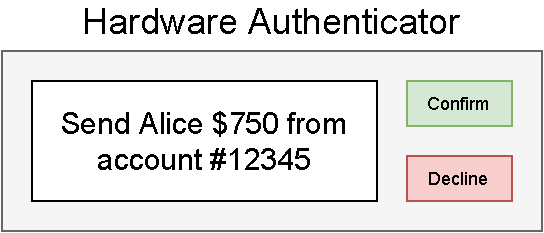
\includegraphics[width=10cm]{authenticator_drawio}
  \caption{User interface of hardware authenticator.}

  %% \centering
  %% \defsvgwidth{\columnwidth}
  %% \input{./images/authenticator_drawio.pdf_tex}
  %% \caption{User interface of hardware authenticator.}
\end{figure}

This message contains enough information such that the user is fully informed of the operation they are about to perform. They can then make the educated judgment for whether to confirm the operation or not. In the adversarial event that Alice were in fact malicious and the monetary transfer is actually intended for Bob, the user should notice this discrepancy in the authentication message and decline the operation on the hardware authenticator. 

The goal of transaction authentication is to prevent the adversary from launching unsolicited operations on behalf of the user and causing fraudulence or damage. The operations that matter will require this additional authentication which the adversary cannot falsify as per the threat model --- the hardware device is assumed secure. This is a safe assumption because the hardware device is specialized to perform only this authentication process and nothing more. Ideally, it should have a minimal attack surface that is vetted by security specialists. 

When the user authorizes this high-risk operation on their hardware authenticator, the message is cryptographically signed by the authenticator and sent back to the verifying end where it gets checked. Only then, upon successful verification is the operation performed. 

Which operations get protected is entirely at the discretion of the administrator of the web service. There is no clear-cut formula on what to protect, but candidate high-risk operations could include, but are not limited to, deleting one's account, transferring money, managing administrative permissions, publishing important software releases, etc. 


%% 
%% \iffalse

%% A security mechanism needs to protect against a stronger threat model in order to further harden a website's security. The threat model can be extended to where most of the transmission chain: the host computer, the operating system, web-browser, network and any other intermediate system may be compromised. And even under such a far-reaching threat model, the security mechanism must prevent unauthorized adversarial operation. What is assumed secure includes only the server code and hardware authenticator, as well as the entire registration event.

%% Traditional two-factor authentication may be simply extended as proposed by the WebAuthn specification \cite{TODO-WebAuthn} released by the World-Wide-Web Consortium (W3C) to work within this new and more restrictive threat model to defend against the class of vulnerabilities not covered by traditional two-factor authentication. This extension is called transaction authentication (txAuthn), and its goal is to enable "high-risk" operations to be individually authenticated by the user's hardware authenticator, despite the user being already logged in.

%% More specifically, when the user tries to issue some high-risk operation, they will be prompted with a message displayed on their paired hardware authenticator. The message is specific to the operation the user is trying to do, and should contain enough information needed for the user to verify that this is indeed the correct operation they want to perform. Upon acceptance by the user, the message is cryptographically signed by the hardware authenticator and sent back to the server where it gets verified, and only then, upon successful verification, is the operation performed.

%% A website, which assumes the more advanced threat model as described, would use transaction authentication to prevent any high-risk operations from being maliciously issued on behalf of the user. Such high-risk operations include, but are not limited to, deleting one's account, transferring money, managing administrative permissions, publishing important software releases, etc. 

%% For example, a bank website could require that monetary transfers exceeding \$500 must be transaction authenticated. In such a case, a possible authentication message that the user would have to confirm could resemble ``Send Alice \$750 from account \#12345''. This message contains enough information such that the user is fully informed as to what operation they are performing. Additionally, in the event that Alice is malicious and the transaction was actually intended for Bob, the user should notice this discrepancy in the authentication message and decline the operation on the hardware authenticator. 

%% \fi
%% 

%% 
%% \iffalse
%% The security benefits brought by transaction authentication to a web service would have a very tangible effect on the website's overall security. Client-side users of the application would have more faith that the website is operating correctly and not doing anything unauthorized at an adversary's request. Administrators of the website would rest more peacefully knowing that even if an adversary got access to their admin panel, they would not be able to do much damage as the critical operations require authentication from a physical hardware devices. And in general as a whole business, greater security would curb unnecessary losses due to hacker exploits and bolster greater trust in the general public's eye.
%% \fi
%% 

\section{Status Quo of Transaction Authentication}\label{Sec:StatusQuo}

Although WebAuthn describes transaction authentication in its protocol specification, no service or hardware authenticator has support for it. Apart from not being integrated into real-world applications, there also has been no investigation into the implications of where transaction authentication fits well, where it is inhibitory or unnecessary, what it takes to support transaction authentication in a web service and any software system designs that would help with integrating and configuring WebAuthn for an existing service.

%% 
%% \iffalse
%% In every case, there is what appears to be an almost standard practice for how WebAuthn gets used and integrated into a web service.
%% \fi
%% 

There are several publicly available codebases in the form of demo applets and libraries that work with WebAuthn \cite{webauthn-online-examples} to illustrate how it can be used in a website. A website typically consists of a frontend and a backend. The frontend is the web code that runs in the user's web-browser and is the origin of all of the user's requests when interacting with the website. The backend consists of the server code and database store that executes the user's requests from the frontend. A web service using WebAuthn would have the frontend issue the WebAuthn requests and have the backend contain the WebAuthn library code to verify those requests and permit the operation if everything passes. Such approach to integrating WebAuthn has a number of practical downsides. 

%% 
%% \iffalse
%% Although this is a straightforward approach and is reasonable for a small applet web service, it begins to suffer when used on a larger codebase where the backend is complicated. 
%% \fi
%% 

Firstly, the backend architecture might not even lend itself well to the control flow of the WebAuthn specification. In order to validate a WebAuthn request, multiple HTTP requests need to be sent back and forth between the frontend and backend. This may not be handled well by the backend if it was built under the assumption that there is only one HTTP request per operation.

Secondly, the integration of WebAuthn transaction authentication into a backend web service tends to be challenging for larger web services. The handler code for each operation is spread throughout the codebase, so it is difficult to keep track of what is secured and where in the code it is. Also, it requires a strong overall understanding of the web service code, which comes with its own set of challenges and slow development speed.

Lastly, in the extreme, albeit unlikely case, the WebAuthn backend may not even be accessible to the software developer if it is, for example, a closed-source API backend. In this case it is impossible to integrate WebAuthn into such a backend.

\section{Thesis Contributions}

There are three major contributions of this thesis. 

\begin{enumerate}[nosep]

\item A firewall system design for integrating WebAuthn transaction authentication into a new or existing web service.

\item Three distinct case studies showcasing the WebAuthn firewall. Each case study observed a class of web service and was used to test the limits of the usability of the firewall.

\item A discussion on the beneficial use cases for transaction authentication, when it makes sense to be applied and when not.

\end{enumerate}

%% 
%% \iffalse
%% A second contribution is the use of the firewall in three distinct case studies.  The last contribution is a discussion on proper (and improper) usage of WebAuthn transaction authentication.
%% \fi
%% 

\subsection{WebAuthn Firewall}

Firstly, it must be emphasized that WebAuthn is simply a protocol specification. Implementation details are not bound to any one way, as long as they comply with the protocol's details. However, the code demos of WebAuthn unanimously integrate it into their applet services in the same intrusive manner. They import a WebAuthn library \cite{webauthn-library} directly into the codebase perform the necessary checks and validation in the backend.

\begin{figure}[h]
  \centering
  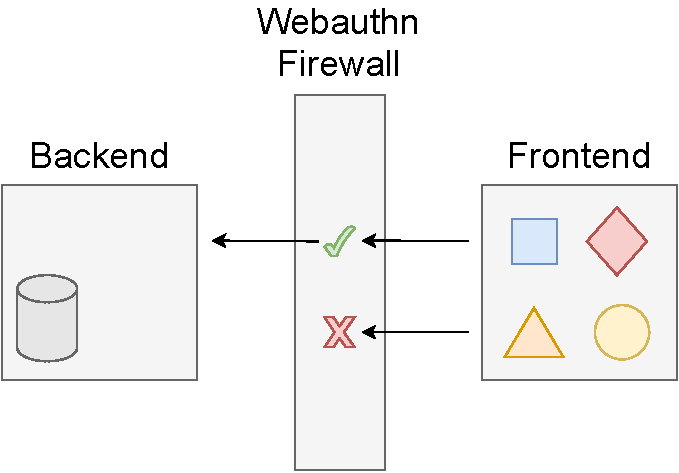
\includegraphics[width=12cm]{firewall_drawio}
  \caption{Basic depiction of WebAuthn firewall functionality.}
\end{figure}

This thesis proposed an alternative method for integrating WebAuthn, namely as a Web Application Firewall (WAF). This firewall monitors and filters HTTP traffic sent from the frontend to the backend. Any requests that the firewall deems as needing WebAuthn transaction authentication are stopped and processed by it. The firewall validates the WebAuthn transaction, complying with the protocol. And if all succeeds, it lets the request pass on through to the backend. As far as the backend is concerned, it is unaware that a firewall exists between it and the frontend. 

With the WebAuthn firewall approach, the backend has to be minimally, if at all, modified to support WebAuthn transaction authentication. Although the frontend still needs to be modified to produce the WebAuthn transaction authentication requests as it is the origin of all of the user's operations, the firewall approach lends itself better to integrating WebAuthn into a new or existing web service. It is less intrusive than the traditional library-based method and consolidates all of the WebAuthn related code in one place. As a result, it is less error-prone and easier to configure. 

%% 
%% \iffalse
%% . Needless to say, such a system design 
%% \fi
%% 

%% TODO: Is mentioning that the firewall is its own application, independent of the frontend or backend, worthwhile?

%% 
%% \iffalse
%% Additionally, the WebAuthn firewall is independent of the frontend and backend. 
%% \fi
%% 

The WebAuthn firewall presented in this thesis goes beyond simply providing a description and base functionality. It supplies the software engineer with useful defaults and a domain specific language (DSL) to configure the firewall. Namely with a short configuration, the engineer can adapt the firewall to parse and understand whatever input request format the web service uses. Additionally, with only a few lines of code per HTTP route, they can also specify that the route gets checked with transaction authentication and what the authentication message should be in order to pass as valid for that operation. 

%% 
%% \iffalse
%% The firewall handles the back-and-forth HTTP requests required for WebAuthn authentication. 

%% So it is much easier for the software engineer to organize and control what operations need transaction authentication and how exactly they get secured. 
%% \fi
%% 

%% 
%% \iffalse
%% % TODO: Are there demos for txAuthn or just WebAuthn. I think the latter only
%% Despite no major applications of WebAuthn, there are several publicly available codebases in the form of demo applets and libraries that work with WebAuthn \cite{TODO-WebAuthn-codebases-from-WebAuthn-website}. In every case, there is what appears to be an almost standard practice for how WebAuthn gets used and integrated into a service. A website typically consists of a frontend and a backend. The frontend is the web code that runs in the user's web-browser and is the origin of all of the user's requests when interacting with the website. The backend consists of the server code and database store that actually operates the website. Traditionally a web service using WebAuthn would have the frontend issue the WebAuthn requests and have the backend contain the code to verify those requests and permit the operation if everything passes. The principal contribution of this thesis demonstrates that there are alternative methods to using and integrating WebAuthn.
%% \fi
%% 

\subsection{Case Studies}

\begin{figure}[h]
  \centering
  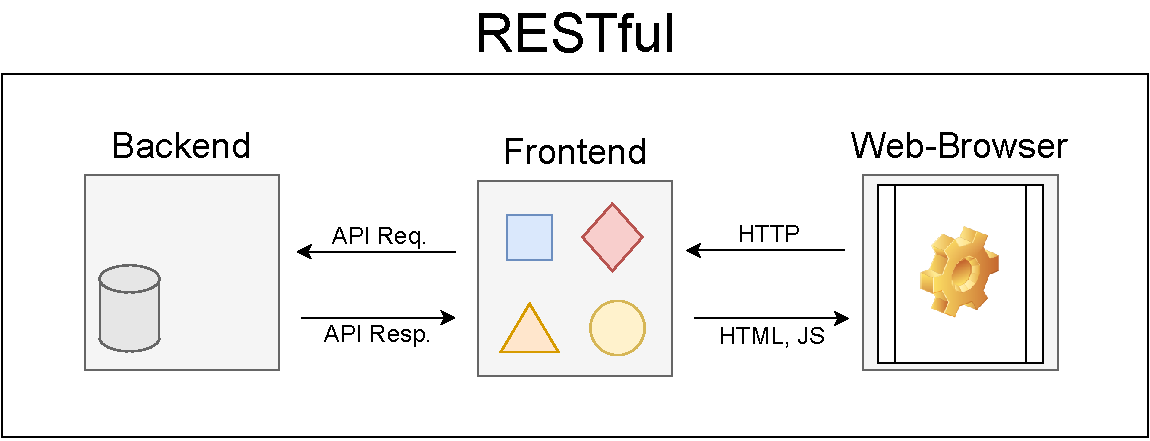
\includegraphics[width=14cm]{RESTful_drawio}
  \caption{The architecture design of a RESTful web application.}
  \label{Fig:CaseStudiesRESTful}
\end{figure}

\begin{figure}[h]
  \centering
  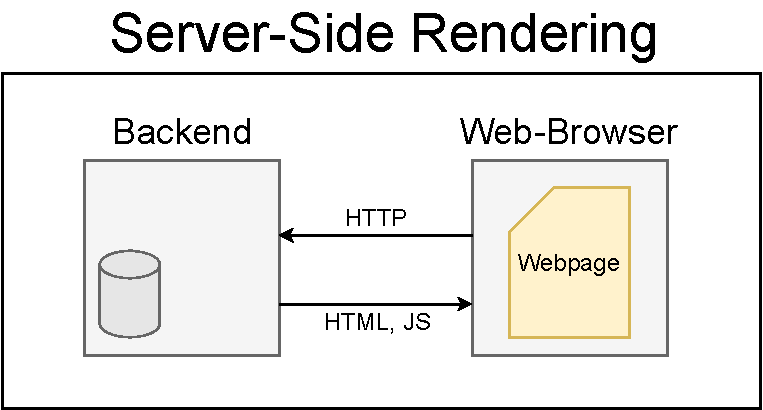
\includegraphics[width=8cm]{ServerSide_drawio}
  \caption{The architecture design of a server-side rendering web application.}
  \label{Fig:CaseStudiesServerSide}
\end{figure}

Three separate case studies demonstrate how the WebAuthn firewall secures different architectures of web applications with WebAuthn transaction authentication. The web applications studied cover the RESTful design paradigm and the more traditional server-side rendering paradigm. The two RESTful applications studied are Conduit \cite{conduit}, a simple blog website, and Calypso \cite{calypso}, a frontend admin panel for WordPress. As illustrated in Figure~\ref{Fig:CaseStudiesRESTful}, the RESTful paradigm is where the webpage frontend and web-server backend are two separate programs. The frontend performs the rendering visible to the user, and whenever it needs to fetch information or has to perform some server operation, it communicates via a pre-established API to the web-server, which executes those requests. 

The server-side rendering application studied is Gogs \cite{gogs}, a self-hosted Git service much like GitHub \cite{github}. Figure~\ref{Fig:CaseStudiesServerSide} depicts the server-side rendering paradigm, where every operation the user performs on the webpage gets sent over to the server as a form POST request. In return, the server responds with a whole new webpage, complete with all of the HTML and JavaScript code to be displayed directly on the user's web-browser.

%% 
%% \iffalse
%% . In return, everything that the user sees gets rendered on the server and is sent back as HTML code to be displayed directly by the user's web-browser.
%% \fi
%% 

These case studies stress test the flexibility and configurability of the WebAuthn firewall. They were critical in establishing what parameters and configurable knobs the firewall should provide. They are also used to evaluate how tangible the improvements are for using the firewall in a service rather than more traditionally integrating WebAuthn transaction authentication intrusively. 

%% 
%% \iffalse
%% Lines of code, complexity, configurability, and integration difficulty are all evaluation criteria which support the use of the WebAuthn firewall over the traditional method.
%% \fi
%% 

\subsection{Other WebAuthn Possibilities}

The thesis also gives insights into best practices relating to utilizing WebAuthn transaction authentication to secure various classes of problems. Researching transaction authentication reveals clear use cases where it lends itself well to secure, some use cases which are doable to secure, but not optimal, and lastly some use cases which cannot be protected at all by transaction authentication. 

%% 
%% \iffalse
%% There is future work that builds on from some of the insights provided by this research. web service routes can be analyzed to verify there is no way to subvert any protected routes. Also transaction authentication can be used to lessen how much code in the transmission chain must be trusted, to provide an even stricter threat model than the one assumed for the WebAuthn firewall. 
%% \fi
%% 

%% 
%% \iffalse
%% \subsection{WebAuthn Status Quo}

%% Firstly, it must be emphasized that WebAuthn is simply a protocol specification. Implementation details are not bound to any one way, as long as they comply with the protocol's details. However, the code demos of webauthn unanimously integrate it into their applet services in the same intrusive manner. They import a webauthn library in one of the many supported languages \cite{TODO-webauthn-libraries} that performs the various validity and authentication checks along the webauthn specification. Then directly in the applications codebase, they invoke the library where it webauthn security is needed. This is a very straightforward coding practice and is very reasonable for a small applet web service. However, the same approach begins to suffer when used on a larger codebase when the backend is complicated and its architecture might not even lend itself well to the control flow of the webauthn specification. In order to validate a webauthn request, multiple HTTP requests need to be sent back and forth between the frontend and backend. This may not be handled well by the backend if it was built under the assumption that one HTTP request per operation. In other cases, the backend is fully inaccessible because it is part of a closed-source software project. 

%% \subsection{Overview of Contributions}

%% An alternative method for integrating webauthn is as a Web Application Firewall (WAF). This firewall monitors and filters HTTP traffic sent from the frontend to the backend. Any requests that the firewall deems as needing further webauthn transaction authentication get stopped. The firewall handles the back-and-forth HTTP requests required for webauthn authentication. And if all succeeds, it lets the request pass on through to the backend. As far as the backend is concerned, it is virtually unaware that a firewall exists between it and the frontend performing the webauthn validation. Under such webauthn firewall approach, the backend has to be minimally, if at all, modified to support webauthn transaction authentication. The frontend still needs to be modified to produce the webauthn transaction authentication requests as it is the origin of all of the user's operations. Needless to say, such a system design lends itself much better for integrating webauthn into a new or existing web service. It is much less intrusive than the traditional library-based method. As a result, it is much less error-prone and easier to configure. Additionally, the webauthn firewall is independent of the frontend and backend. So it is much easier for the software engineer to organize and control what operations need transaction authentication and how exactly they get secured. 

%% The webauthn firewall presented in this thesis goes beyond simply providing base functionality. It supplies the software engineer with useful defaults and a powerful domain specific language (DSL) to configure the firewall. Namely with a short configuration, the engineer can adapt the firewall to parse and understand whatever input request format the web service uses. Additionally, with only a few lines of code per HTTP route, they can also specify that the route gets checked with transaction authentication and what the authentication message should be in order to pass as valid for that operation. 

%% Furthermore, case studies demonstrate how the webauthn firewall secures three different architectures of web applications with webauthn transaction authentication. The web applications studied cover the RESTful design paradigm and the more traditional server-side rendering paradigm. The RESTful paradigm is where the webpage frontend and web-server backend are two separate programs. The frontend performs the rendering visible to the user, and whenever it needs to fetch information or has to perform some server operation, it communicates via a standardized API to the web-server which executes those requests. The server-side rendering paradigm is where every operation the user performs on the webpage gets requested to the server directly. In return, everything that the user sees gets rendered on the server and is sent back as HTML code to be displayed directly by the user's web-browser.

%% These case studies stress test the flexibility and configurability of the webauthn firewall. They were critical in establishing what parameters and configurable knobs the firewall should provide. They are also used to evaluate how tangible the improvements are for using the firewall in a service rather than more traditionally integrating webauthn transaction authentication intrusively. Lines of code, complexity, configurability, and integration difficulty are all evaluation criteria which support the use of the webauthn firewall over the traditional method.

%% Beyond describing the webauthn firewall, the thesis will also give insights into best practices relating to utilizing webauthn transaction authentication to secure various classes of problems. Researching transaction authentication revealed clear use cases where it lends itself well to secure, some use cases which are doable to secure, but not optimal, and lastly some use cases which are not protected at all be transaction authentication. There is future work that builds on from some of the insights provided by this research. web service routes can be analyzed to verify there is no way to subvert any protected routes. Also transaction authentication can be used to lessen how much code in the transmission chain must be trusted, to provide an even stricter threat model than the one assumed for the webauthn firewall. 
%% \fi
%% 

%% 
%% \iffalse
%% in order a protected operation to be processed by the web-server, it must be 

%% but it is not void of vulnerabilities

%% with only a few lines of code per HTTP route, the engineer can adapt the firewall to parse and understand whatever input request format the web service uses. 

%% specify whether the route gets checked with transaction authentication and what the authentication message should be to pass as valid for that operation. 

%% Each  how well it can support a variety of different web applications, each with different 
%% \fi
%% 

\subsection{Source Code}

The source code of the WebAuthn firewall and case studies is publicly available at \url{https://github.com/JSmith-BitFlipper/webauthn-firewall-proxy} under the MIT License. Cheers! 

\section{Thesis Outline}

The thesis body is containing in the following chapters. Chapter~\ref{Chap:RelatedWork} discusses the related work and background pertinent to this research. Chapter~\ref{Chap:WebauthnTransactionAuthentication} describes the WebAuthn transaction authentication protocol in detail. Chapter~\ref{Chap:WebauthnFirewallDesign} outlines the design of the WebAuthn firewall. Chapter~\ref{Chap:WebauthnFirewallImplementation} discusses the implementation details of the novel components of the firewall. Chapter~\ref{Chap:CaseStudies} explains the case studies of the WebAuthn firewall. Chapter~\ref{Chap:Evaluations} contains the experiments and evaluation metrics for the firewall. Chapter~\ref{Chap:DiscussionAndFutureWork} opens a discussion of supplemental notes uncovered over the course of this research. Finally, Chapter~\ref{Chap:Conclusion} concludes this thesis.
